%%%%%%%%%%%%%%%%%%%%%%%%%%%%%%%%%%%%%%%%%%%%%%%%%%%%%%%%%%%%%%%%%%%%%%%%%%%%%%%%
%
% Plantilla para libro de texto de matemáticas.
%
% Esta plantilla ha sido desarrollada desde cero para el proyecto apuntesDGIIM
% de LibreIM.
%
%	Copyright (C) 2019 LibreIM
%
% This program is free software: you can redistribute it and/or modify
% it under the terms of the GNU Affero General Public License as
% published by the Free Software Foundation, either version 3 of the
% License, or (at your option) any later version.
% This program is distributed in the hope that it will be useful,
% but WITHOUT ANY WARRANTY; without even the implied warranty of
% MERCHANTABILITY or FITNESS FOR A PARTICULAR PURPOSE.  See the
% GNU Affero General Public License for more details.
% You should have received a copy of the GNU Affero General Public License
% along with this program.  If not, see <https://www.gnu.org/licenses/>.
%
%%%%%%%%%%%%%%%%%%%%%%%%%%%%%%%%%%%%%%%%%%%%%%%%%%%%%%%%%%%%%%%%%%%%%%%%%%%%%%%%

% ------------------------------------------------------------------------------
% CONFIGURACIÓN BÁSICA DEL DOCUMENTO
% ------------------------------------------------------------------------------

\documentclass[fontsize=12pt]{scrartcl}
\usepackage[spanish, es-tabla, es-lcroman, es-noquoting, es-minimal]{babel}
\usepackage{graphicx}

% ------------------------------------------------------------------------------
% CONFIGURACIÓN DE ASIGNATURA
% ------------------------------------------------------------------------------

\usepackage{config}

% ------------------------------------------------------------------------------
% TIPOGRAFÍA
% ------------------------------------------------------------------------------

% Tipografía personalizada
\usepackage[bitstream-charter]{mathdesign}
\usepackage[scale=0.88, type1]{FiraSans}
\usepackage[scale=0.88, type1]{FiraMono}
\usepackage[T1]{fontenc}

% Microtype
\usepackage[activate={true, nocompatibility}, final, tracking=true,factor=1100, stretch=10, shrink=10]{microtype}
\SetTracking{encoding={*}, shape=sc}{0}

% Matemáticas en sans serif si es necesario
\usepackage{sansmath}
\newif\IfInSansMode
\let\oldsf\sffamily
\renewcommand*{\sffamily}{\oldsf\sansmath\InSansModetrue}

% ------------------------------------------------------------------------------
% DISEÑO DE PÁGINA
% ------------------------------------------------------------------------------

% Márgenes
\usepackage[bottom=3.125cm, top=2.5cm, left=2.5cm, right=4.5cm, marginparwidth=70pt]{geometry} 

% Párrafos
\linespread{1.1}
\setlength{\parindent}{12pt}
\setlength{\parskip}{0pt}

% Cabeceras
\usepackage[automark]{scrlayer-scrpage}
\clearpairofpagestyles
\chead{\leftmark}
\cfoot*{\pagemark}

% No mostrar cabecera en páginas de sección
\usepackage{xpatch}
\xpretocmd{\section}{\vspace*{1cm}\thispagestyle{plain}}{}{}

% Páginas de color para portada
\usepackage{pagecolor}
\usepackage{afterpage}

% ------------------------------------------------------------------------------
% ENTORNOS PERSONALIZADOS
% ------------------------------------------------------------------------------

\usepackage[theorems, skins, breakable]{tcolorbox}

\tcolorboxenvironment{nth}{
	blanker,
	breakable,
	left=12pt,
	before skip=12pt,
	after skip=12pt,
	borderline west={2pt}{0pt}{500},
	before upper={\parindent 12pt},
}

\tcolorboxenvironment{nprop}{
	blanker,
	breakable,
	left=12pt,
	before skip=12pt,
	after skip=12pt,
	borderline west={2pt}{0pt}{300},
	before upper={\parindent 12pt},
}

\tcolorboxenvironment{ncor}{
	blanker,
	breakable,
	left=12pt,
	before skip=12pt,
	after skip=12pt,
	borderline west={2pt}{0pt}{300},
	before upper={\parindent 12pt},
}

\tcolorboxenvironment{ndef}{
	skin=enhancedmiddle jigsaw,
	frame hidden,
	colback=50,
	breakable = true,
	break at = -6pt,
	top = 4pt,       % Estos márgenes están un poco a ojo
	bottom = 4pt,
	left= 8pt,
	right = 8pt,
	before skip=8pt, % Normalmente dejamos 12pt, pero
	after skip=8pt,  % aquí tenemos espacio adicional por el fondo
	no borderline,
	borderline west={2pt}{0pt}{500},
	borderline east={2pt}{0pt}{50},
	before upper={\parindent 12pt},
}

\tcolorboxenvironment{ejer}{
	skin=enhancedmiddle jigsaw,
	frame hidden,
	colback=50,
	breakable = true,
	break at = -6pt,
	top = 4pt,       % Estos márgenes están un poco a ojo
	bottom = 4pt,
	left= 8pt,
	right = 8pt,
	before skip=8pt, % Normalmente dejamos 12pt, pero
	after skip=8pt,  % aquí tenemos espacio adicional por el fondo
	no borderline,
	borderline west={2pt}{0pt}{500},
	borderline east={2pt}{0pt}{50},
	before upper={\parindent 12pt},
}

% ------------------------------------------------------------------------------
% LISTINGS
% ------------------------------------------------------------------------------

\renewcommand{\lstlistingname}{Listado}

\lstset{
  frame=lines,
  rulecolor=\color{black},
  framerule=1pt,
  numbers=left,
  belowcaptionskip=1\baselineskip,
  basicstyle=\ttfamily\color{black},
  keywordstyle=\bfseries\color{700},
  commentstyle=\color{300},
  stringstyle=\color{500},
  numberstyle=\color{black},
  breaklines=true,
  showstringspaces=false,
  tabsize=2,
}

% ------------------------------------------------------------------------------
% PANDOC
% ------------------------------------------------------------------------------

% Paquetes y comandos que utiliza Pandoc para compilar

\usepackage{hyperref}
\hypersetup{
	colorlinks=true,
	linkcolor=500,
}
\usepackage{longtable}
\usepackage{booktabs}
\usepackage{stmaryrd}

\providecommand{\tightlist}{%
	\setlength{\itemsep}{0pt}\setlength{\parskip}{0pt}}
	
\newcommand{\passthrough}[1]{#1}

\DeclareOldFontCommand{\bf}{\normalfont\bfseries}{\mathbf}

% Ajuste del tamaño de las imágenes
\makeatletter
\def\maxwidth{\ifdim\Gin@nat@width>\linewidth\linewidth
\else\Gin@nat@width\fi}
\makeatother
\let\Oldincludegraphics\includegraphics
\renewcommand{\includegraphics}[1]{\Oldincludegraphics[width=\maxwidth]{#1}}

%%%%%%%%%%%%%%%%%%%%%%%%%%%%%%%%%%%%%%%%%%%%%%%%%%%%%%%%%%%%%%%%%%%%%%%%%%%%%%%%
% ------------------------------------------------------------------------------
% COMIENZO DEL DOCUMENTO
% ------------------------------------------------------------------------------
%%%%%%%%%%%%%%%%%%%%%%%%%%%%%%%%%%%%%%%%%%%%%%%%%%%%%%%%%%%%%%%%%%%%%%%%%%%%%%%%

\begin{document}

% ---------------------------------------------------------------------------
% PORTADA EXTERIOR
% ---------------------------------------------------------------------------

\newpagecolor{500}
\begin{titlepage}
	\noindent
	\setlength\fboxsep{0cm}
	\parbox[t]{\textwidth}{
			\raggedright
			\fontsize{50pt}{50pt}\selectfont\sffamily\color{white}{
			  \textbf{\asignatura}
      }
	}

	\vfill

	\noindent
	\parbox[b]{\textwidth}{
		\raggedright 
		\sffamily\large\color{white}
		{\Large \autor }\\[4pt]
		\grado\\
		\universidad\\[4pt]
		\texttt{\enlaceweb}
	}

\end{titlepage}
\restorepagecolor

% ---------------------------------------------------------------------------
% PÁGINA DE LICENCIA
% ---------------------------------------------------------------------------

\thispagestyle{empty}
\null
\vfill

\noindent
\parbox[b]{0.7\textwidth}{
  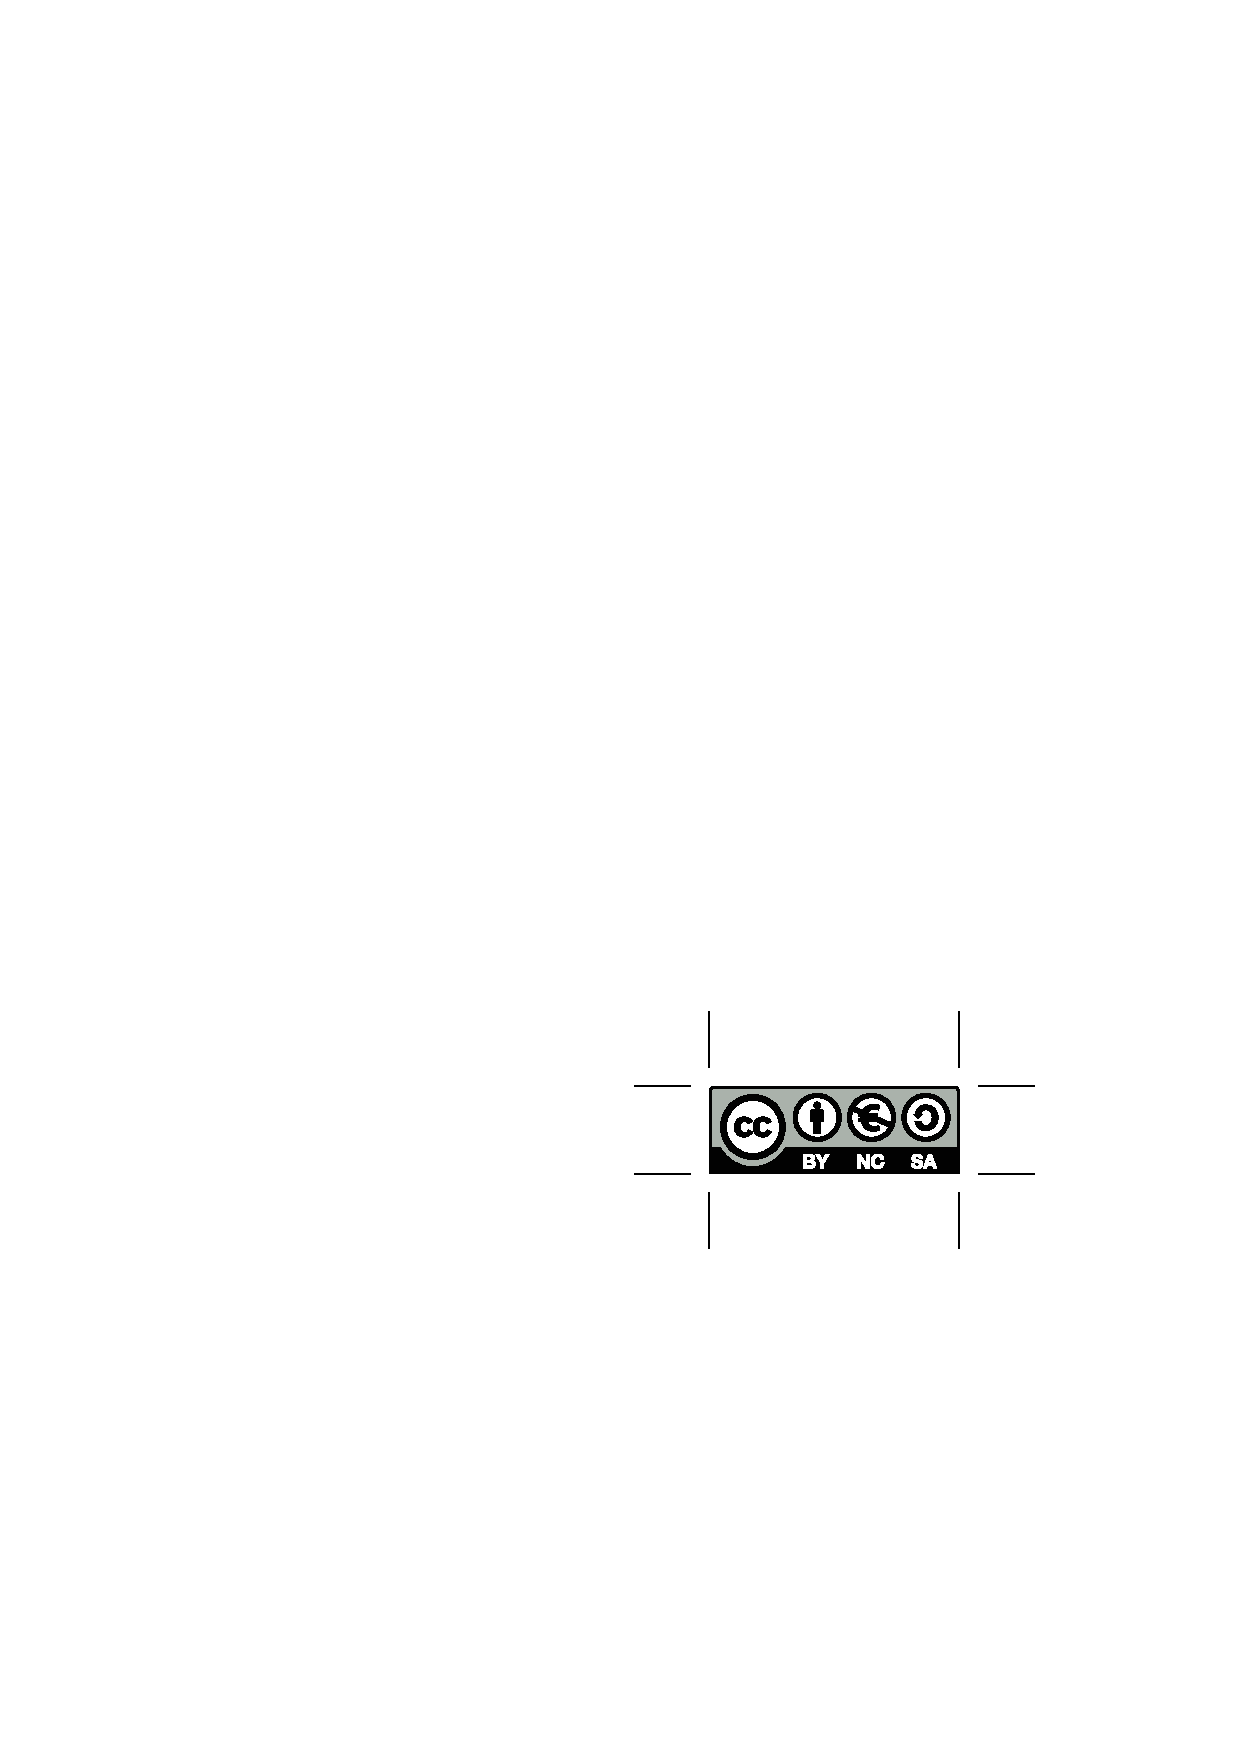
\includegraphics{by-nc-sa.pdf}\\[4pt]
  \raggedright
  \sffamily
  {\large Este libro se distribuye bajo una licencia CC BY-NC-SA 4.0.}\\[4pt]
  Eres libre de distribuir y adaptar el material siempre que reconozcas a los autores originales del documento, no lo utilices para fines comerciales y lo distribuyas bajo la misma licencia.\\[4pt]
  \texttt{creativecommons.org/licenses/by-nc-sa/4.0/}
}

% ---------------------------------------------------------------------------
% PORTADA INTERIOR
% ---------------------------------------------------------------------------

\begin{titlepage}

	\noindent
	\parbox[t]{\textwidth}{
			\raggedright
			\fontsize{50pt}{50pt}\selectfont\sffamily\color{500}{
			  \textbf{\asignatura}
      }
	}

	\vfill

	\noindent
	\parbox[b]{\textwidth}{
		\raggedright
		\sffamily\large
		{\Large \autor}\\[4pt]
		\grado\\
		\universidad\\[4pt]
		\texttt{\enlaceweb}
	}

\end{titlepage}

% ---------------------------------------------------------------------------
% ÍNDICE
% ---------------------------------------------------------------------------

\thispagestyle{empty}
\tableofcontents
\newpage

% ---------------------------------------------------------------------------
% PANDOC
% ---------------------------------------------------------------------------

$if(abstract)$
\begin{abstract}
$abstract$
\end{abstract}
$endif$

$for(include-before)$
$include-before$

$endfor$
$if(toc)$
{
$if(colorlinks)$
\hypersetup{linkcolor=$if(toccolor)$$toccolor$$else$black$endif$}
$endif$
\setcounter{tocdepth}{$toc-depth$}
\tableofcontents
}
$endif$
$if(lot)$
\listoftables
$endif$
$if(lof)$
\listoffigures
$endif$
$body$

$if(natbib)$
$if(bibliography)$
$if(biblio-title)$
$if(book-class)$
\renewcommand\bibname{$biblio-title$}
$else$
\renewcommand\refname{$biblio-title$}
$endif$
$endif$
\bibliography{$for(bibliography)$$bibliography$$sep$,$endfor$}

$endif$
$endif$
$if(biblatex)$
\printbibliography$if(biblio-title)$[title=$biblio-title$]$endif$

$endif$

% ---------------------------------------------------------------------------
% CONTENIDO
% ---------------------------------------------------------------------------

$for(include-after)$

$include-after$

$endfor$

\end{document}
